
\begin{figure*}
\centering
\subfloat[Figure A][Access to the network using a signaling server]{
  
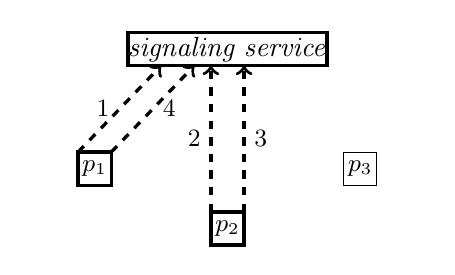
\begin{tikzpicture}[scale=1.2]

\newcommand\X{40pt};
\newcommand\Y{18pt};

\draw( 1.5*\X, 0); %% spacing
\draw(-1.5*\X, 0); %% spacing

\draw[fill=white,very thick](0*\X, 0*\Y) 
node{\emph{signaling service}} +(-30pt,-5pt) rectangle +(30pt,5pt);

\small
\draw[->,dashed, very thick](-5 -1*\X, 5-2*\Y) --
node[anchor=east]{1} (-20pt,-5pt);
\draw[->,dashed, very thick]( 5 -1*\X, 5-2*\Y) --
node[anchor=west]{4} (-10pt,-5pt);

\draw[->,dashed, very thick](-5pt,  5-3*\Y) --
node[anchor=east]{2}(-5pt,-5pt);
\draw[->,dashed, very thick](5pt , 5-3*\Y) --
node[anchor=west]{3} (5pt,-5pt);


\draw[fill=white, very thick]
(-1*\X,-2*\Y) node{$p_1$} +(-5pt,-5pt) rectangle +(5pt,5pt);
\draw[fill=white, very thick]
(0*\X, -3*\Y) node{$p_2$} +(-5pt,-5pt) rectangle +(5pt,5pt);
\draw[fill=white] (1*\X, -2*\Y) node{$p_3$} +(-5pt,-5pt) rectangle +(5pt,5pt);

\end{tikzpicture}

% \begin{tikzpicture}
% \matrix (m) [matrix of math nodes,row sep=4em,column sep=4em] {
% \node(ss)[draw]{signaling}; & \node(p3)[draw]{p3}; \\
% \node(p1)[draw]{p1}; & \node(p2)[draw]{p2}; \\
% };
% \path[->]
%   (p2) edge[dashed] node[fill=white]{1:emit} (ss)
%   (p3) edge[dashed] node[fill=white,bend left]{2:pull} (ss)
%   (p3) edge[dashed, bend right] node[fill=white]{3:accept} (ss)
%   (p2) edge[dashed,bend left] node[fill=white]{4:pull} (ss)
%   (p3) edge[<->,thick] node[fill=white,right]{5:connected} (p2);
% \end{tikzpicture}}
\hspace{20pt}
\subfloat[Figure B][\label{fig:webrtcB}Use the network itself to establish new
connections]{
  
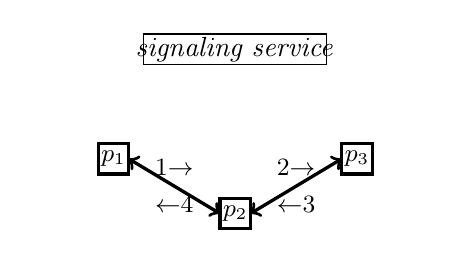
\begin{tikzpicture}[scale=1.1]

\newcommand\X{40pt};
\newcommand\Y{18pt};

\draw(1.7*\X, 0); %% spacing
\draw(-1.7*\X, 0); %% spacing

\draw[fill=white](0*\X, 0*\Y)
node{\emph{signaling service}} +(-30pt,-5pt) rectangle +(30pt,5pt);

\small
\draw[<->, very thick](5-1*\X,-2*\Y)--
node[anchor=south]{1$\rightarrow$}
node[anchor=north]{$\leftarrow$4}(-5pt,-3*\Y);
\draw[<->, very thick](5pt,-3*\Y)--
node[anchor=south]{2$\rightarrow$}
node[anchor=north]{$\leftarrow$3}(-5+1*\X,-2*\Y);

\draw[fill=white, very thick]
(-1*\X,-2*\Y) node{$p_1$} +(-5pt,-5pt) rectangle +(5pt,5pt);
\draw[fill=white, very thick]
(0*\X, -3*\Y) node{$p_2$} +(-5pt,-5pt) rectangle +(5pt,5pt);
\draw[fill=white, very thick]
(1*\X, -2*\Y) node{$p_3$} +(-5pt,-5pt) rectangle +(5pt,5pt);

\end{tikzpicture}

% \begin{tikzpicture}
% \matrix (m) [matrix of math nodes,row sep=4em,column sep=4em] {
% \node(ss)[draw]{signaling}; & \node(p3)[draw]{p3}; \\
% \node(p1)[draw]{p1}; & \node(p2)[draw]{p2}; \\
% };
% \path[->]
%   (p1) edge[dashed,bend left] node[fill=white]{1:emit} (p2)
%   (p2) edge[dashed,bend left] node[fill=white,left]{2:emit/p1} (p3)
%   (p3) edge[dashed,bend left] node[fill=white,right]{3:accept/p1} (p2)
%   (p2) edge[dashed,bend left] node[fill=white]{4:accept} (p1)
%   (p1) edge[<->,thick] (p2)
% %  (p1) edge[<->,thick,bend left] (p3)
%   (p2) edge[<->,thick]  (p3);

% \end{tikzpicture}}
\hspace{20pt}
\subfloat[Figure C][Resulting network overlay]{
  
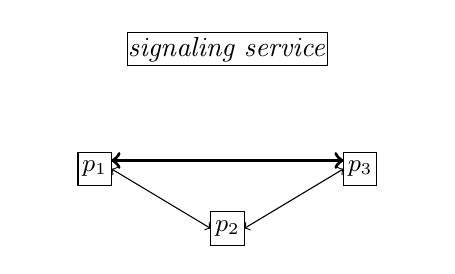
\begin{tikzpicture}[scale=1.2]

\newcommand\X{40pt};
\newcommand\Y{18pt};

\draw(1.5*\X, 0); %% spacing
\draw(-1.5*\X, 0); %% spacing

\draw[fill=white](0*\X, 0*\Y)
node{\emph{signaling service}} +(-30pt,-5pt) rectangle +(30pt,5pt);

\small
\draw[<->](5-1*\X,-2*\Y)--(-5pt,-3*\Y);
\draw[<->](5pt,-3*\Y)--(-5+1*\X,-2*\Y);
\draw[<->, very thick](5 - 1*\X, 2.5 -2*\Y)--(-5+1*\X, 2.5 -2*\Y);

\draw[fill=white]
(-1*\X,-2*\Y) node{$p_1$} +(-5pt,-5pt) rectangle +(5pt,5pt);
\draw[fill=white]
(0*\X, -3*\Y) node{$p_2$} +(-5pt,-5pt) rectangle +(5pt,5pt);
\draw[fill=white]
(1*\X, -2*\Y) node{$p_3$} +(-5pt,-5pt) rectangle +(5pt,5pt);

\end{tikzpicture}


% \begin{tikzpicture}
% \matrix (m) [matrix of math nodes,row sep=4em,column sep=4em] {
% \node(ss)[draw]{signaling}; & \node(p3)[draw]{p3}; \\
% \node(p1)[draw]{p1}; & \node(p2)[draw]{p2}; \\
% };
% \path[->]
%   (p1) edge[<->,thick] (p2)
%   (p1) edge[<->,thick] (p3)
%   (p2) edge[<->,thick]  (p3);
% \end{tikzpicture}}
\caption{\label{fig:webrtc}Creating an overlay network on top of WebRTC.}
\end{figure*}


\section{Related work}
\label{sec:relatedwork}


WebRTC allows real-time communication from browser-to-browser even
with complex network settings such as firewall, proxies or Net Address
Translation (NAT). However, WebRTC do not manage addressing nor
routing. To establish a connection, browsers have to exchange offers
and acknowledges through a mediator that can be mails, dedicated
signaling service~\footnote{\url{http://peerjs.com/}}, or existing
WebRTC connections~\footnote{\url{http://github/P ??}}. In
figure~\ref{fig:webrtc}, $p2$ wants to connect $p3$. $p2$ push an
offer ticket to a signaling service\footnote{Many signaling services
  can exist}. $p3$ pulls the offers, stamps it and pushes it back to
the signaling service. Next, $p2$ pulls the stamped ticket and
establish a bidirectional connection with $p3$. The same protocol is
used for connecting $p1$ to $p2$. In this state, it is possible to
establish a connection between $p1$ and $p3$ without the mediation of
the signaling service. $p1$ pushes an offer ticket to $p2$.  as $p2$
is already connected to $p1$, it forwards the offer to $p3$ and
piggyback $p1$ to the offer. $p3$ stamps the ticket and sends it back
to $p2$ that forwards it to $p1$. Notices that If $p2$ crashes between
step 2 and 3, then connection will fail even if an alternative route
exists as webRTC does not manage routing.  

Using signaling services and existing WebRTC connections allow to
deploy random peer sampling protocols~\cite{jelasity2004peer} easily
on browsers that can run on mobile phones or tablets connected to
mobile networks. In this context, it is crucial to keep the number of
connections as low as possible in order to limit the traffic and
ressource consumption. 

Random peer sampling protocols~\cite{jelasity2004peer} provide each
peer with a partial view $\mathcal{P}$ of the network membership
$\mathcal{N}$. They populate the partial views with the reference of
peers chosen at random among $\mathcal{N}$ following a uniform
distribution using local knowledge only. Their goal is to converge to
an overlay network exposing properties similar to random
graphs~\cite{erdos1959random}. They efficiently provide connectedness,
robustness, messages dissemination etc. A wide variety of gossip-based
protocols use random peer sampling (e.g. topology
management~\cite{voulgaris2005epidemic, jelasity2009tman,
  dabek2004vivaldi}).

Representatives of random peer sampling
protocols~\cite{voulgaris2005cyclon, eugster2003lightweight,
  tolgyeski2009adaptive} use a fixed-size partial view.  Thus, they
have to know \emph{a priori} the maximum order of magnitude of the
network size to set their appropriate parameters. These decisions
cannot be safely retracted afterwards. For this reason, the partial
views are commonly oversized compared to the actual network
size. Consequently, it is possible for a browser to maintain 10
connections with others while only 6 were required. In WebRTC context,
we need a dynamic peer sampling service able to adapt to number of
participants.

Network size estimators can be used to introduce adaptivity in peer
sampling. These approaches either use
\begin{inparaenum}[(i)]
\item sampling techniques~\cite{mane05network, ganesh2007peer,
    kostoulas2007active} which analyze a network subset and deduce the network
  size using probabilistic functions,
\item sketching techniques~\cite{flajolet2008hyperloglog, baquero2012extrema}
  which use hashing to compress the high amount of data and deduce the network
  size using the collisions,
\item averaging techniques~\cite{jelasity2004epidemic, blasa2011symmetric}
  which use aggregations that converge over exchanges to a value which depends
  of the network size.
\end{inparaenum}
Unfortunately, while they can be very precise in their estimate, they
imply a communication overhead and may have strong assumptions
(e.g. random graph topology). In WebRTC context, adaptivity should
introduce a minimum overhead in peer sampling.

The sole representative of adaptive-by-design random peer sampling is
\SCAMP{}~\cite{ganesh2001scamp,ganesh2003peer} which stands for
SCalable Membership Protocol. Its interesting property lies in its
logarithmically growing partial view sizes meeting the sharp threshold
of connectedness of random
graphs~\cite{erdos1959random}. Nevertheless, \SCAMP{} suffers from
other flaws. In particular, it systematically performs random walks to
establish its connections. In the WebRTC context, each random walk
must be traveled back to finalize the connection establishment as
illustrated in figure~\ref{fig:webrtc}. It drastically impacts on the
\SCAMP{} failure probability of establishing a connection. Indeed, let
$P_f$ the probability of either the peer or the link between the
latter and the next peer crashes/disconnects when it holds the
traveling message, without any possible recovery. Let $P_E$ the
probability that a connection establishment cannot be
completed. Without three-way handshake, $P_E$ is straightforward:
\begin{equation} P_{E,\,1way}^{Scamp}=1-(1- P_f)^{k+1} \end{equation} where $k$
is the number of hops before the end of the random walk with a minimum of $2$
hops. On the other hand, in the handshaking context, the message must travel
back to its origin in order to be completed. As consequence, when a
subscription travels through a peer or a link, they are not allowed to fail
until the subscription travels back. Thus, we obtain:
\begin{align} P_{E,\,3way}^{Scamp} &=1 - ((1-P_f)^{2(k+1)} (1-P_f)^{2k}
                                     \ldots (1-P_f)^2) \nonumber \\
                                   &=1-(1-P_f)^{k^2+3k+2}
\end{align}
The complexity class of the \SCAMP{} failure rate increases leading to a quick
degenerating number of connections over time. This behaviour endangers the
connectedness of network.

Building an adaptive-by-design random peer sampling that meet WebRTC
constraints raises the following scientific problem:

\begin{problem}
  Let $t$ be an arbitrary time frame, let $\mathcal{N}^t$ be the network
  membership at that given time $t$ and let $\mathcal{P}_x^t$ be the partial
  view of peer $p_x \in \mathcal{N}^t$.  A cost-efficient random peer sampling,
  especially when three-way handshaking is involved, should provide the
  following best-case properties:
  \begin{center}
    Partial view size: \hfill
    $\forall p_x \in \mathcal{N}^t,\, |\mathcal{P}_x^t| = \Theta (\ln
    |\mathcal{N}^t|)$
  \end{center}
  \begin{center}
    Connection establishment: \hfill $O(1)$
  \end{center}
  \begin{center}
    Convergence speed: \hfill $\Theta(\exp \, t^{-1})$
  \end{center}
\end{problem}

%%% Local Variables:
%%% mode: latex
%%% TeX-master: "../paper"
%%% End:
